\chapter{Steps of a Data-Driven Approach}
\chapterintrobox{
A \acrlong{dd} prognostics approach (an approach that uses system's operation data, like historic monitoring data, to build a model that is used to predict remaining usefil life) must go through multiple stages---from data acquisition to estimating remaining service life. In this chapter, these different steps will be discussed in detail.
}

\section{Data acquisition}
\label{sec:data-acquisition}
A signal is a function that conveys information about the behavior of a system or the attributes of a phenomenon. Signals occur naturally and are also synthesized. A signal is not necessarily an electrical quantity. However, to perform activities such as synthesizing, transporting, recording, analyzing and modifying signals, it is often convenient to use a signal in the form of an electrical quantity \cite{Priemer1990}.

Data acquisition is a process of capturing and storing different types of monitoring data (i.e. signals) from various sensors installed on the monitored equipment. It is the first machine prognostics process, which provides basic condition monitoring information for subsequent processes. A data acquisition system is composed of sensors, data transmission devices and data storage devices \cite{Lei2018}. Condition monitoring data is very versatile. It can be vibration data, acoustic data, oil analysis data, temperature, pressure, humidity, weather or environmental data, and so on. Different sensors, such as micro-sensors, ultrasonic sensors and acoustic emission sensors have been designed to collect different types of data. Wireless technologies, such as Bluetooth, have provided a cost-effective alternative to data communication \cite{Jardine2006}.

Although research on advanced concepts such as wireless sensor networks and energy harvesting to power autonomous sensors is ongoing, data acquisition (sensors) and manipulation are now fairly well established. Consequently, much of the research in this discipline focuses on analyzing the data obtained to extract information \cite{Tinga2014}. Because this discipline is well developed, many new data acquisition facilities and techniques have been designed and applied in modern industries. These powerful and versatile facilities have made data acquisition for \acrshort{phm} implementation more practical and feasible\cite{Lei2016}.

\section{Features Extraction}
The data-driven prognostics approach is mainly used when it is difficult to understand the physical behaviour of a complex system. Understanding the behaviour and interaction of the different elements that lead to machine degradation is the starting point for developing a physical model for prognostics.
On the other hand, this approach uses condition monitoring data to implicitly model its behaviour. The models used in the data-driven approach use monitoring data to model complex behavior and capture complex models, but they are considered as black boxes: they do not necessarily provide insight into the process.
In general, the performance of these models depends on the quality of the input (i.e. data). The human part cannot perform the task that the model performs, but processing the input data can significantly increase the results. This processing is necessary because the sensor data on which the model is based is usually redundant, noisy and incomplete, and there are many reasons for these imperfections.

Feature extraction is an important pre-processing step in the development process of machine learning models and directly influences the performance of the model. Therefore, this step must be performed carefully in order to extract meaningful features from the raw data. Vibration data contains very useful information about the state of the system, but requires extensive pre-processing before it can be used as input data for a specific model. This chapter describes some of the signal processing techniques used in traditional vibration analysis, but in this context they will be used as feature extractors for a neural network architecture.

\subsection{Signal analysis}
Signal processing is the study and analysis of stored signals to reveal their properties-which may not be apparent at first glance-using a set of algorithms and techniques. In the context of condition monitoring, these properties revealed by signal processing may be indicative of the health of the machine.
Signal processing is a well-established and mature sub-domain of electrical engineering, with many techniques and algorithms proposed in the literature.

Signal processing can be divided into three categories: \textbf{Time-Domain Analysis}, \textbf{Frequency-Domain Analysis} and \textbf{Time--Frequency Analysis}.

\subsection{Temporal Analysis}.
The original measurements of signals that are usually repeatedly sampled between predefined time intervals are in the form of a time series. Thus, time domain analysis is directly based on the original measurement \cite{Lei2016}.

\subsection{Frequency-Domain Analysis}
Frequency domain analysis is based on signals transformed in the frequency domain. The advantage of frequency-domain analysis over time-domain analysis is its ability to decompose the original signals into a series of frequency components. The most commonly used frequency domain analysis is spectrum analysis using Fast Fourier Transform (FFT). The main idea of spectrum analysis is to isolate and locate certain frequency components of interest related to the fault characteristics of \cite{Lei2016a} machines.

\subsection{Time--Frequency Analysis}
The problem with time-domain analysis and frequency-domain analysis is that each has no information on the other (time-domain analysis has no information on the frequency-domain, and frequency-domain analysis has no information on the time-position).

Thus, time--frequency domain analysis, which
studies measurement signals in the time and frequency domains, has been applied to the analysis of non-stationary measurement signals. Time--frequency analysis describes the characteristics of measurement signals in two-dimensional functions of time and frequency to better reveal machine failure modes.

Figure \ref{fig:signal-processing} presents different techniques for each type of analysis:

\begin{figure}[h]
    \centering
	\begin{tikzpicture}
\tikzstyle{element}=[draw,rectangle]
\tikzstyle{entity}=[fill=gray!20,align=center, text width=8em]
\node[element] (fe) {Signal processing};


\node[element,below = 1.6em of fe] (fd) {Frequency analysis};
\node[element,left = of fd] (td) {Time series analysis};
\node[element,right = of fd] (tfd) {Time--Frequency analysis};

\node[entity,below =.5em of td] (stat) {Statistics-based};
\node[entity,below =.5em of stat] (arm) {Autoregressive Model};
\node[entity,below =.5em of arm] (arma) {ARMA Model};
\node[entity,below =.5em of arma] (tsa) {Time Synchronous Average};

\node[entity,below =.5em of fd] (fft) {Fourier Transform};
\node[entity,below =.5em of fft] (cep) {Cepstrum};
\node[entity,below =.5em of cep] (hil) {Hilbert Transform};\node[entity,below =.5em of hil] (env) {Envelope Analysis};


\node[entity,below =.5em of tfd] (stft) {Short-Time Fourier Transform};
\node[entity,below =.5em of stft] (wt) {Wavelet Transform};
\node[entity,below =.5em of wt] (hht) {Hilbert-Huang Transform};
\node[entity,below =.5em of hht,align=center, text width=8em] (emd) {Empirical Mode Decomposition};

\draw[->,>=angle 60] (fe.south) -- ++(0,0) -- ++(0,-.8em) -| (td);
\draw[->,>=angle 60] (fe.south) -| (fd);
\draw[->,>=angle 60] (fe.south) -- ++(0,0) -- ++(0,-.8em) -| (tfd);
\end{tikzpicture}

    \caption{Techniques de traitement du signal dans les différents domaines}
    \label{fig:signal-processing}
\end{figure}

\subsection{Fourier analysis}
Fourier analysis, also called harmonic analysis, of a periodic signal $x(t)$ is the decomposition of the series into summation of sinusoidal components, where each sinusoid has a specific amplitude and phase.

The Fourier transform (FT) of a signal $x(t)$ can be mathematically given by equation \ref{equation:fourier-transform}:

\begin{equation}
    X(w) = \int_{-\infty}^{\infty}x(n)e^{-jwt}dt
    \label{equation:fourier-transform}
\end{equation}

In practical applications of digital signal processing where signals are discrete in time rather than continuous (e.g. vibration analysis) a discretized version called discrete fourier transform (DFT) is used instead, it is expressed mathematically by equation \ref{equation:discrete-fourier-transform}:

\begin{equation}
    X(w) = \sum_{-\infty}^{\infty}x(t)e^{-jwt}dt
    \label{equation:discrete-fourier-transform}
\end{equation}

Fast Fourier transform (FFT) is an effective algorithm used to implement DFT in computers. Figure \ref{figure:fft} shows a signal in its waveform (or time domain) and its corresponding spectrum (frequency domain) obtained using FFT algorithm. The spectrum shows the frequency components present in the signal:

\begin{figure}[H]
    \centering
    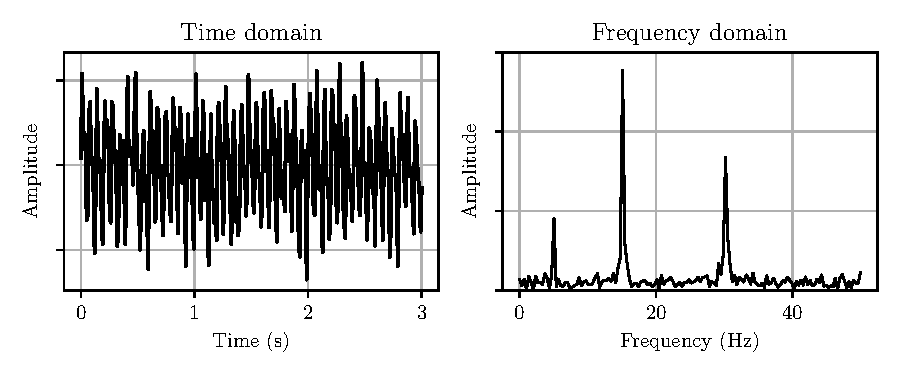
\includegraphics{figures/fft.pdf}
    \caption{Signal in the time domain and its fast Fourier transform}
    \label{figure:fft}
\end{figure}

\subsection{Wavelet transform}
Wavelet transform is also a spectral analysis tool, like Fourier transform. The main difference is that Fourier transform decomposes the signal into sinusoidal components, but wavelet transform decomposes it into a set of oscillatory functions called \textbf{wavelets}. Unlike sinusoids, wavelets are localized in time, thus wavelet transform doesn't only provide information about the frequency present in a signal but also the time of their occurence. Wavelet transform is a much better solution than Fourier transform when studying non-linear non-stationary signals (i.e. its frequency components vary with time).

Figure \ref{fig:time-frequency-plane} shows the difference in time and frequency resolutions between different methods. In the waveform, the signal has absolute resolution in time and zero resolution in frequency. Fourier transform on the contrary transforms the signal totally into the frequency domain, therefore it has absolute resolution in frequency but no resolution in time. Short-time Fourier transform is calculated identically to fourier transform but it is performed on separate segments of the original signal to preserve some resolution in time. Wavelet transform on the other hand exhibits a high time resolution for high frequencies and high frequency resolution for low frequencies:

\begin{figure}[H]
    \centering
    \begin{subfigure}{.35\textwidth}
	\centering
	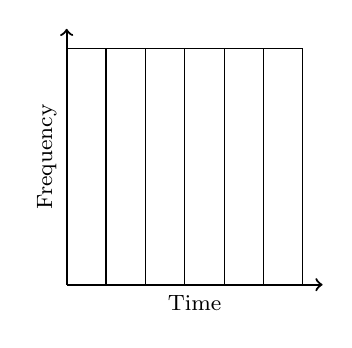
\begin{tikzpicture}
	\draw (0,0) -- (3,0);
	\draw (3,0) -- (3,-3);
	\path[thick, ->]  (0,-3) edge node[below] {\footnotesize Time} (3.25,-3)  ;
	\path[thick, ->] (0,-3) edge node[above, rotate=90] {\footnotesize Frequency} (0,.25)  ;
	
	\draw (.5,0) -- (.5,-3);
	\draw (1,0) -- (1,-3);
	\draw (1.5,0) -- (1.5,-3);
	\draw (2,0) -- (2,-3);
	\draw (2.5,0) -- (2.5,-3);
	
	\draw (3,0) -- (3,-3);
	\end{tikzpicture}
	\caption{Waveform}
\end{subfigure}%
\begin{subfigure}{.35\textwidth}
	\centering
	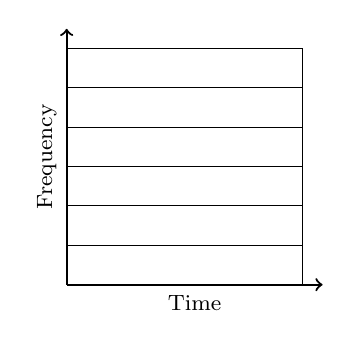
\begin{tikzpicture}
	\draw (0,0) -- (3,0);
	\draw (3,0) -- (3,-3);
	\path[thick, ->]  (0,-3) edge node[below] {\footnotesize Time} (3.25,-3)  ;
	\path[thick, ->] (0,-3) edge node[above, rotate=90] {\footnotesize Frequency} (0,.25)  ;
	
	\draw (0,-.5) -- (3,-.5);
	\draw (0,-1) -- (3,-1);
	\draw (0,-1.5) -- (3,-1.5);
	\draw (0,-2) -- (3,-2);
	\draw (0,-2.5) -- (3,-2.5);
	
	\end{tikzpicture}
	\caption{Fourier Transform}
\end{subfigure}

\medskip

\begin{subfigure}{.35\textwidth}
	\centering
	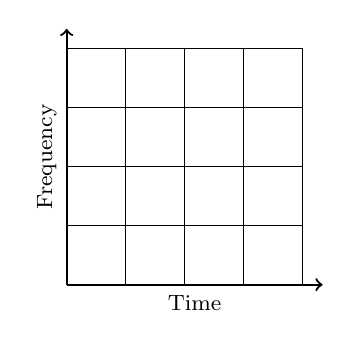
\begin{tikzpicture}
	
	\draw (0,0) -- (3,0);
	\draw (3,0) -- (3,-3);
	\path[thick, ->]  (0,-3) edge node[below] {\footnotesize Time} (3.25,-3)  ;
	\path[thick, ->] (0,-3) edge node[above, rotate=90] {\footnotesize Frequency} (0,.25)  ;
	
	\draw (0.75,0) -- (0.75,-3);
	\draw (0,-0.75) -- (3,-0.75);
	\draw (1.5,0) -- (1.5,-3);
	\draw (2.25,0) -- (2.25,-3);
	\draw (0,-1.5) -- (3,-1.5);
	%	\draw (3,0) -- (3,-3);
	\draw (0,-2.25) -- (3,-2.25);
	
	\end{tikzpicture}
	\caption{Short-Time Fourier}
\end{subfigure}%
\begin{subfigure}{.35\textwidth}
	\centering
	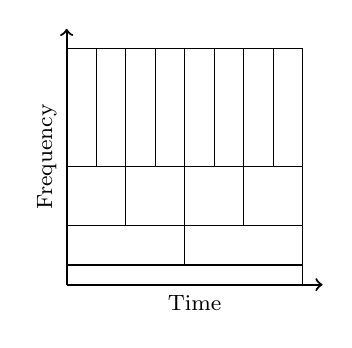
\begin{tikzpicture}
	\draw (0,0) -- (3,0);
	\draw (3,0) -- (3,-3);
	\path[thick, ->]  (0,-3) edge node[below] {\footnotesize Time} (3.25,-3)  ;
	\path[thick, ->] (0,-3) edge node[above, rotate=90] {\footnotesize Frequency} (0,.25)  ;
	\draw (0,-1.5) -- (3,-1.5);
	\draw (0,-2.25) -- (3,-2.25);
	
	\draw (0,-2.75) -- (3,-2.75);
	\draw (1.5,0) -- (1.5,-2.75);
	
	\draw (0.75,0) -- (0.75,-2.25);
	\draw (2.25,0) -- (2.25,-2.25);
	
	\draw (0.375,0) -- (0.375,-1.5);
	\draw (1.125,0) -- (1.125,-1.5);
	\draw (1.875,0) -- (1.875,-1.5);
	\draw (2.625,0) -- (2.625,-1.5);
	\end{tikzpicture}
	\caption{Wavelet Transform}
\end{subfigure}


\begin{comment}
%BIGGER VERSION

\begin{subfigure}{.4\textwidth}
	\centering
	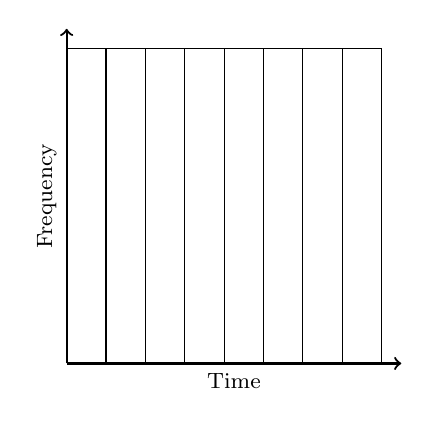
\begin{tikzpicture}
	\draw (0,0) -- (4,0);
	\draw (4,0) -- (4,-4);
	\path[thick, ->]  (0,-4) edge node[below] {\footnotesize Time} (4.25,-4)  ;
	\path[thick, ->] (0,-4) edge node[above, rotate=90] {\footnotesize Frequency} (0,.25)  ;
	
	\draw (.5,0) -- (.5,-4);
	\draw (1,0) -- (1,-4);
	\draw (1.5,0) -- (1.5,-4);
	\draw (2,0) -- (2,-4);
	\draw (2.5,0) -- (2.5,-4);
	\draw (3,0) -- (3,-4);
	\draw (3.5,0) -- (3.5,-4);
	\end{tikzpicture}
	\caption{Waveform}
\end{subfigure}%
\begin{subfigure}{.4\textwidth}
	\centering
	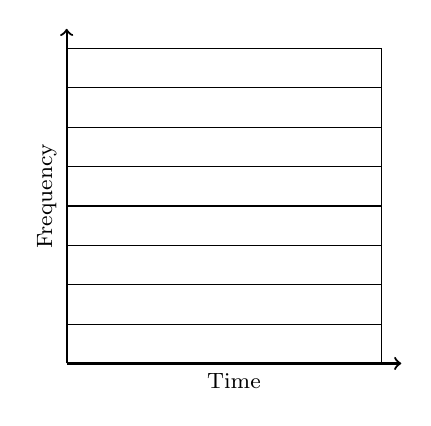
\begin{tikzpicture}
	\draw (0,0) -- (4,0);
	\draw (4,0) -- (4,-4);
	\path[thick, ->]  (0,-4) edge node[below] {\footnotesize Time} (4.25,-4)  ;
	\path[thick, ->] (0,-4) edge node[above, rotate=90] {\footnotesize Frequency} (0,.25)  ;
	
	\draw (0,-.5) -- (4,-.5);
	\draw (0,-1) -- (4,-1);
	\draw (0,-1.5) -- (4,-1.5);
	\draw (0,-2) -- (4,-2);
	\draw (0,-2.5) -- (4,-2.5);
	\draw (0,-3) -- (4,-3);
	\draw (0,-3.5) -- (4,-3.5);
	\end{tikzpicture}
	\caption{Fourier Transform}
\end{subfigure}

\medskip

\begin{subfigure}{.4\textwidth}
	\centering
		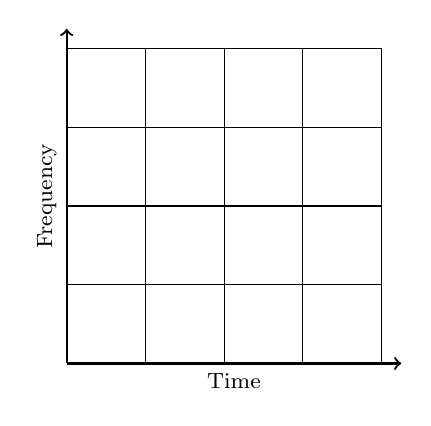
\begin{tikzpicture}
	
	\draw (0,0) -- (4,0);
	\draw (4,0) -- (4,-4);
	\path[thick, ->]  (0,-4) edge node[below] {\footnotesize Time} (4.25,-4)  ;
	\path[thick, ->] (0,-4) edge node[above, rotate=90] {\footnotesize Frequency} (0,.25)  ;
	
	\draw (1,0) -- (1,-4);
	\draw (0,-1) -- (4,-1);
	\draw (2,0) -- (2,-4);
	\draw (0,-2) -- (4,-2);
	\draw (3,0) -- (3,-4);
	\draw (0,-3) -- (4,-3);
	
	\end{tikzpicture}
	\caption{Short-Time Fourier Transform}
\end{subfigure}%
\begin{subfigure}{.4\textwidth}
	\centering
	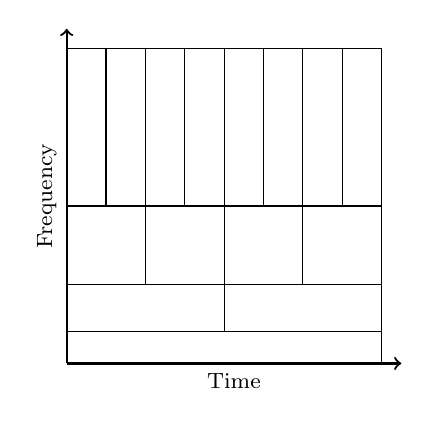
\begin{tikzpicture}
		\draw (0,0) -- (4,0);
		\draw (4,0) -- (4,-4);
		\path[thick, ->]  (0,-4) edge node[below] {\footnotesize Time} (4.25,-4)  ;
		\path[thick, ->] (0,-4) edge node[above, rotate=90] {\footnotesize Frequency} (0,.25)  ;
		\draw (0,-2) -- (4,-2);
		\draw (0,-3) -- (4,-3);
	
		\draw (0,-3.6) -- (4,-3.6);
		\draw (2,0) -- (2,-3.6);
	
		\draw[-] (1,0) -- (1,-3);
		\draw[-] (3,0) -- (3,-3);
	
		\draw[-] (.5,0) -- (.5,-2);
		\draw[-] (1.5,0) -- (1.5,-2);
	
		\draw[-] (2.5,0) -- (2.5,-2);
		\draw[-] (3.5,0) -- (3.5,-2);
	\end{tikzpicture}
	\caption{Wavelet Transform}
\end{subfigure}
\end{comment}
    \caption{Time—frequency resolution plane}
    \label{fig:time-frequency-plane}
\end{figure}

There are a wide variety of wavelets that serve different purposes like Morlet wavelet, Daubechies wavelet and many others.

\begin{figure}[H]
    \centering
    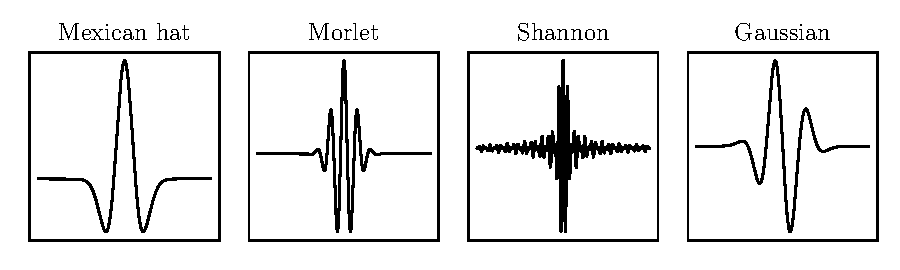
\includegraphics{figures/wavelets.pdf}
    \caption{Different types of wavelets}
    \label{fig:wavelets}
\end{figure}

\subsubsection{Continuous wavelet transform}
Mathematically, continuous wavelet transform is defined by equation \ref{equation:cwt}:

\begin{equation}
    CWT_x^\psi(\tau, s)=\frac{1}{\sqrt{|s|}}\int_{-\infty}^{\infty}x(t)\psi^* \left(\frac{t-\tau}{s}\right)dt
    \label{equation:cwt}
\end{equation}

Where $x(t)$ is the original signal, $\psi^*$ is a function called the \textbf{mother wavelet}; $s$ and $\tau$ are the \textbf{scale} and \textbf{translation} parameters respectively. The original signal is multiplied by the mother wavelet which is scaled using different scales then translated over the signal.

The output of \acrshort{cwt} is a scaleogram like the one in figure \ref{fig:scaleogram} which is a scaleogram (filled contour plot) of vibrations data snapshot of 25ms:

\begin{figure}[H]
    \centering
    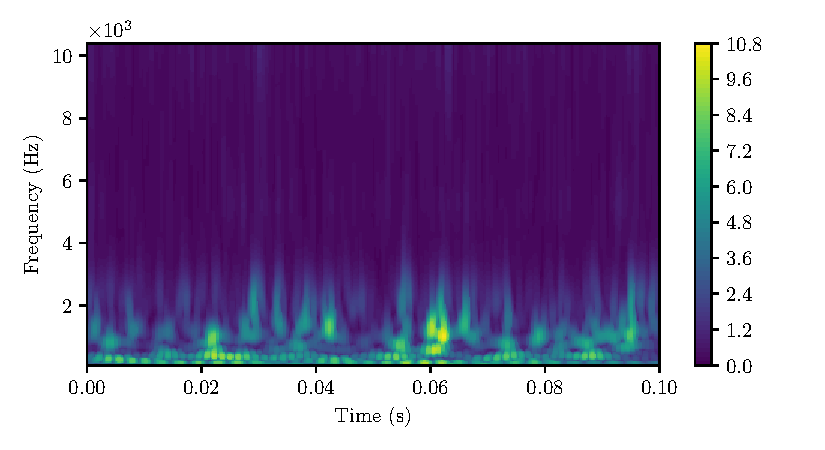
\includegraphics{figures/scaleogram.pdf}
    \caption{Scaleogram of vibration data snapshot}
    \label{fig:scaleogram}
\end{figure}

The x and y axes represent time and frequency respectively. Different colors indicate the power (i.e. amplitude) of each frequency (y-axis) during each instant of time (x-axis) which—unlike Fourier transform—provides information about the frequencies present in the signal and also the instances of time when these frequencies are present.

\subsubsection{Discrete wavelet transform}%
\label{subsub:discrete_wavelet_transform}
In practical applicaions, discrete wavelet transform (DWT) is implemented as a filter bank where the signal is passed therough low- and high-pass filters to obtain \textbf{approximation} and \textbf{decomposition coefficients}. Figure \ref{fig:dwt} shows a DWT with 2 levels of decomposition which yields 2nd order approximation and decomposition coefficients:

\begin{figure}[H]
    \centering
    \begin{tikzpicture}[cell/.style={rectangle,draw, thick,align=center, minimum size=2em,inner sep=5pt}, input/.style={->}]

\node[cell] at (0,0) (xn) {$x[n]$};

\node[cell] at (-1.5,-1.5) (lpf1) {$LPF$};
\node[cell] at (1.5,-1.5) (hpf1){$HPF$};

\node[cell] at (-1.5,-3) (A1) {A1};
\node[cell, below = 1em of hpf1]  (D1) {D1};

\node[cell, below left = 2em of A1] (lpf2) {$LPF$};
\node[cell, below right = 2em of A1] (hpf2){$HPF$};

\node[cell, below = 1em of lpf2]  (A2) {A2};
\node[cell, below = 1em of hpf2]  (D2) {D2};

\draw[->, >=angle 60] (xn) -- ++(0,-1em) -- ++(0,-0.75em) -| (lpf1);
\draw[->, >=angle 60] (xn) -- ++(0,-1em) -- ++(0,-0.75em) -| (hpf1);

\draw[->, >=angle 60] (lpf1) -- (A1);
\draw[->, >=angle 60] (hpf1) -- (D1);

\draw[->, >=angle 60] (A1) -- ++(0,-1em) -- ++(0,-0.8em) -| (lpf2);
\draw[->, >=angle 60] (A1) -- ++(0,-1em) -- ++(0,-0.8em) -| (hpf2);

\draw[->, >=angle 60] (lpf2) -- (A2);
\draw[->, >=angle 60] (hpf2) -- (D2);

\node[] at (3,-0.9) (coord1) {};
\node[] at (3,-3.25) (coord2) {};

\end{tikzpicture}
    \caption{Discrete wavelet transform (DWT) as a filter bank}
    \label{fig:dwt}
\end{figure}

\begin{figure}[H]
    \centering
    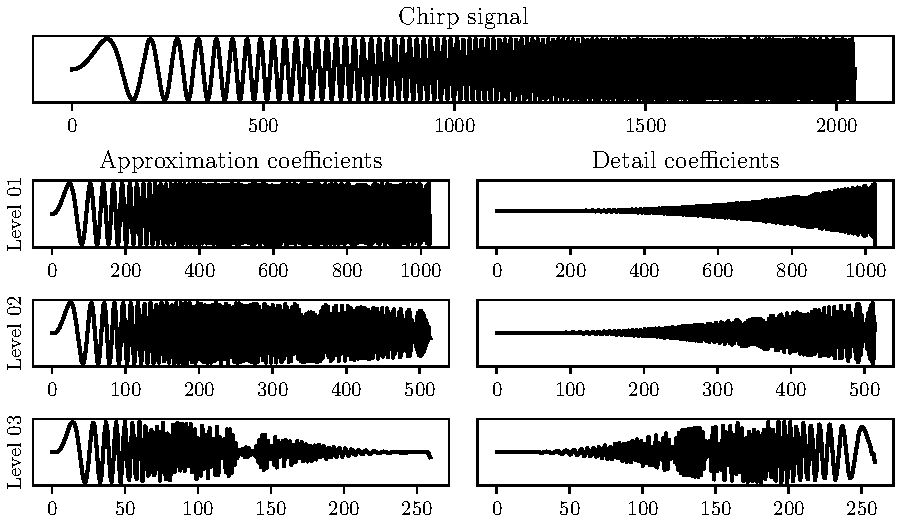
\includegraphics{figures/dwt_chirp.pdf}
    \caption{Level 3 signal decomposition using DWT}
    \label{fig:dwt-chirp-signal}
\end{figure}

DWT returns two sets of coefficients: \textbf{approximation coefficients} associated with the low pass filter and \textbf{detail coefficients} associated with the high pass filter of the DWT. By applying DWT again on the approximation coefficients the next level of decomposition can be obtained. At each level the original signal is downsampled by a factor of 2, this fact imposes a limitation on the possible number of decomposition levels for a given signal.

\subsection{Dimensionality reduction}
\label{section:dimensionality-reduction}
Dimensionality reduction refers to the process of taking high-dimensional data and finding a good representation of this data in a lower dimension while preserving its original characteristics. Dimensionality reduction is performed for feature extraction by finding the main components or for visualization (by reducing the number of dimensions to 2 or 3).
There are many dimensionality reduction techniques and algorithms such as:
\begin{itemize}
    \item Principal Component Analysis (PCA)
    \item Autoencoders
    \item t-Distributed Stochastic Neighbor Embedding (t-SNE)
\end{itemize}

It should be noted that for prognoses, where the data used consist of sensor inputs where each variable has a physical meaning and direct interpretation, performing a dimensionality reduction will give the main components, but the new variables \textit{will lose their physical interpretability} and \textit{shall be treated as abstractions}.


\section{Diagnostics}
Diagnostics is a process of identifying and determining the relationship between the information obtained in the measurement space and the failure modes of the machines in the failure space. Diagnostics consists of three main steps: fault detection, fault isolation and fault identification. Fault detection is the task of indicating whether a fault has already occurred in the monitored machines. Fault isolation consists of finding the component of the fault and the position of the fault. Fault identification is the final step in diagnosis, which attempts to determine the mode and severity of the failure. The three steps are interrelated. This last step is based on the results of the first one and therefore cannot be performed individually \cite{Lei2016b}.

\section{Prognostics}
Diagnosis is the analysis of the later event and prognosis is the analysis of the earlier event. Prognosis is much more effective than diagnosis in achieving performance without stopping production. However, diagnosis is necessary when the prediction of prognostic errors fails and an error occurs \cite{Jardine2006}.
Prognostics are the forecast or prediction of the future performance of a system, this prediction is based on its current state. The prediction is performed using a model, types of prognostic models are already discussed in details in section \ref{section:prognostics-approaches} but the focus of this current discussion is geared towards data-driven models. More concretely, what these models predict is the remaining useful life (\acrshort{rul}) defined in section \ref{section:rul-estimation}. Prognostics models---by estimating \acrshort{rul}---aim at scheduling maintenance actions according to the predictions and production constraints associated with the machine in order to achieve zero unscheduled equipment downtime.

\section{Maintenance decision}
The next and the last step of any prognostics approach is to use the output of the developed model (i.e. predictions, or estimations for the system's \acrshort{rul}) in making better and more accurate preventive maintenance actions. Maintenance decision makers should analyze the outputs of the model prior to taking any actions, since any model has an inherent error associated with its predictions. Usually, data-driven models provide confidence intervals associated with their predictions which must be considered carefully. Also it must be noted that those confidence itervals are reflection of the models certainty of its predictions based on the data provided for the training, in real applications a new unforeseen failure mode can occure which may not have happened before, thus it wasn't provided for the model as part of the data used to consutrct it. This is more or less associated with the ability of different types of models to generalize for new unforeseen data, but in general it is well-known fact that any data-driven model will be less reliable when performing predictions using data that the model didn't see before \cite{Chung2018}. That's why providing quality data that reflects different degradation patterns and fault modes is essential for the model to make more robust and reliable predictions.

\section{Conclusion}
Developing a (data-driven) prognostics model is a process that requires many steps: from data acquisition required to construct the model to employing the model predictions in making better and more accurate maintenance decisions which result in less (or even zero) unscheduled downtime this reduced costs and decreased production loss, the latter being the ultimate goal of all this discussion and prognostics/preventive maintenance literature in general. The focus of this discussion is data-driven models, one of the models that proved great ability in learning complex non-linear patterns in data are neural networks. These models have different architecture depending on the structure of data. They will be presented and explained in details in the next chapter.

\section{Conclusion}
Vibration data are discrete signals sampled at a certain frequency in time. Although they hold so many valuable information about equipment performance, these information are usually not directly observable in the time domain. Digital signal processing techniques offer a way to gain more insights from raw vibration data by converting it to frequency or time–frequency domains where unusual frequency components can indicate development of certain degradation pattern. This chapter introduced several of these techniques like Fourier and Wavelet transforms. A following chapter will present the use of these techniques for extracting features that serve as an input for a neural network that can estimate the remaining useful life.
